\documentclass[10pt]{article}
\usepackage[margin=0.72in]{geometry}
\usepackage[T1]{fontenc}
\usepackage{amsmath}
\usepackage{graphicx}
\usepackage{booktabs}
\usepackage{caption}
\usepackage[colorlinks=true,linkcolor=black,citecolor=black,urlcolor=blue]{hyperref}
\captionsetup{font=small,labelfont=bf}
\setlength{\parskip}{0.45em}
\setlength{\parindent}{0pt}

\title{Response-Surface Constrained Kinetic Analysis of Visible-Light Dye Photodegradation on Nitrogen-Modified TiO$_2$}
\author{Light Skills Synthetic Science Demo}
\date{}

\begin{document}
\maketitle

\begin{abstract}
This synthetic study demonstrates a reproducible environmental-chemistry workflow for visible-light dye photodegradation. A deterministic generator produced 4968 UV-vis time records across 183 experimental conditions covering catalyst formulation, loading, pH, irradiance, and radical-scavenger perturbations. Pseudo-first-order fits recovered an optimum condition using N-TiO2/H2O2 at 0.50 g L$^{-1}$, pH 7.0, and 105 mW cm$^{-2}$, with $k_\mathrm{obs}=0.0296$ min$^{-1}$ and an apparent half-life of 23.4 min. The paper is a workflow demonstration only: it does not claim a real photocatalyst discovery.
\end{abstract}

\textbf{Honesty boundary.} All concentration traces are synthetic and generated by the repository script. The package demonstrates a science-style workflow: data, analysis, figures, references, manuscript, LaTeX source, PDF, and preview.

\section{Introduction}
Semiconductor photocatalysis is a long-running route for light-driven environmental remediation~\cite{fujishima1972,hoffmann1995,pelaez2012}. A realistic computational demonstration should include time-resolved concentration traces, kinetic fitting, design-factor response surfaces, diagnostics, and mechanistic perturbation. This project uses that structure to showcase Light Skills without inventing experimental evidence.

\begin{figure}[htbp]
\centering
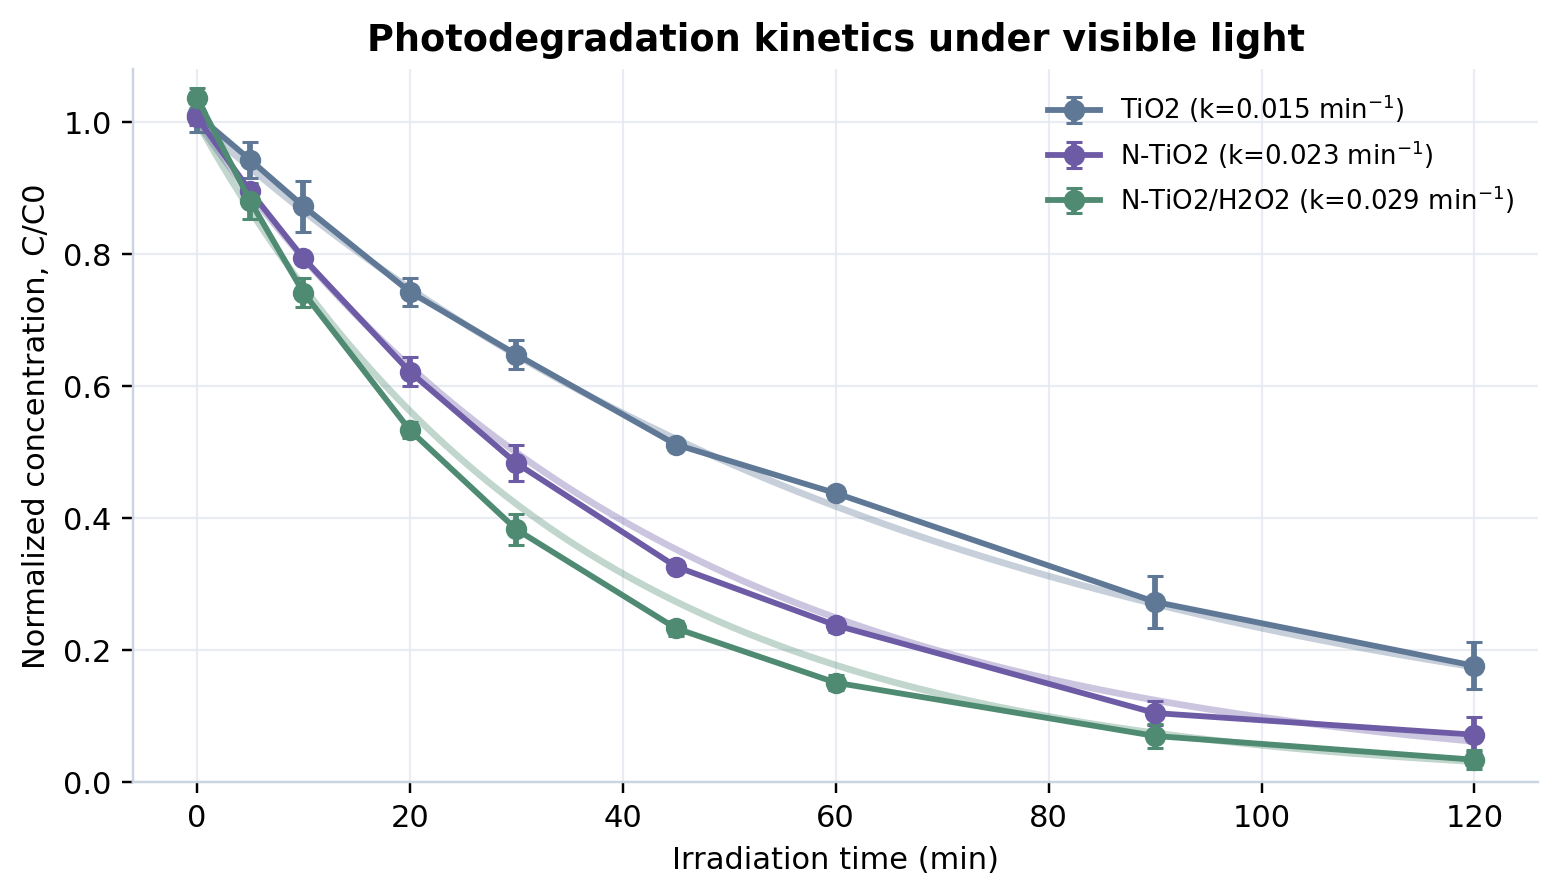
\includegraphics[width=0.96\linewidth]{../figures/figure1_kinetics.png}
\caption{Synthetic visible-light degradation traces at the high-irradiance neutral-pH condition. Markers show replicate means and standard deviations; smooth lines are pseudo-first-order fits.}
\label{fig:kinetics}
\end{figure}

\section{Methods}
Synthetic UV-vis absorbance records were generated for three catalyst formulations, five catalyst loadings, four pH levels, three irradiance settings, and a radical-scavenger panel. Rate constants were estimated by fitting
\[
\ln(C/C_0) = -k_\mathrm{obs}t + b
\]
for each condition. The response surface was summarized for N-TiO$_2$/H$_2$O$_2$ at fixed irradiance. Numerical analysis used NumPy, SciPy, and Matplotlib~\cite{harris2020,virtanen2020,hunter2007}.

\begin{table}[htbp]
\centering
\caption{Bootstrap summaries over synthetic no-scavenger design conditions. Values are demonstration outputs, not measured catalyst performance.}
\begin{tabular}{lrrrr}
\toprule
Catalyst & Mean $k_\mathrm{obs}$ & 95\% CI low & 95\% CI high & $n$ \\
\midrule
N-TiO2/H2O2 & 0.0235 & 0.0227 & 0.0243 & 60 \\
N-TiO2 & 0.0182 & 0.0175 & 0.0189 & 60 \\
TiO2 & 0.0111 & 0.0107 & 0.0114 & 60 \\
\bottomrule
\end{tabular}
\label{tab:catalysts}
\end{table}

\section{Results}
The response surface selected N-TiO2/H2O2 near neutral pH and intermediate catalyst loading as the fastest simulated condition. The top catalyst-family mean was N-TiO2/H2O2 with mean $k_\mathrm{obs}=0.0235$ min$^{-1}$. The analysis is intentionally framed as a synthetic benchmark so that the artifact demonstrates a complete science workflow without overstating evidence.

\begin{figure}[htbp]
\centering
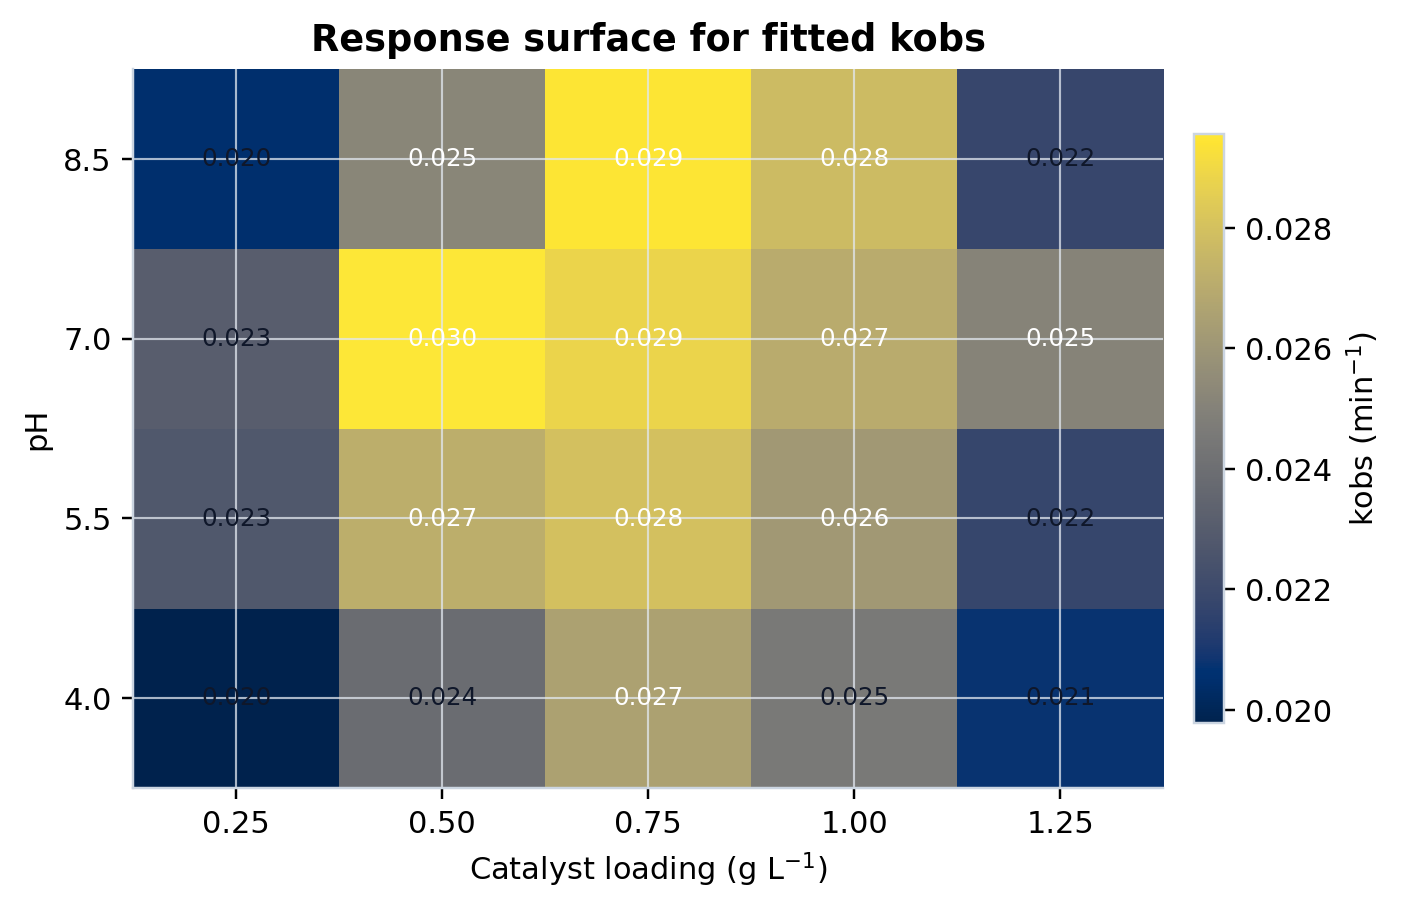
\includegraphics[width=0.78\linewidth]{../figures/figure2_response_surface.png}
\caption{Response surface for fitted $k_\mathrm{obs}$ under N-TiO$_2$/H$_2$O$_2$ at fixed irradiance. The surface is generated from synthetic data.}
\label{fig:surface}
\end{figure}

\begin{figure}[htbp]
\centering
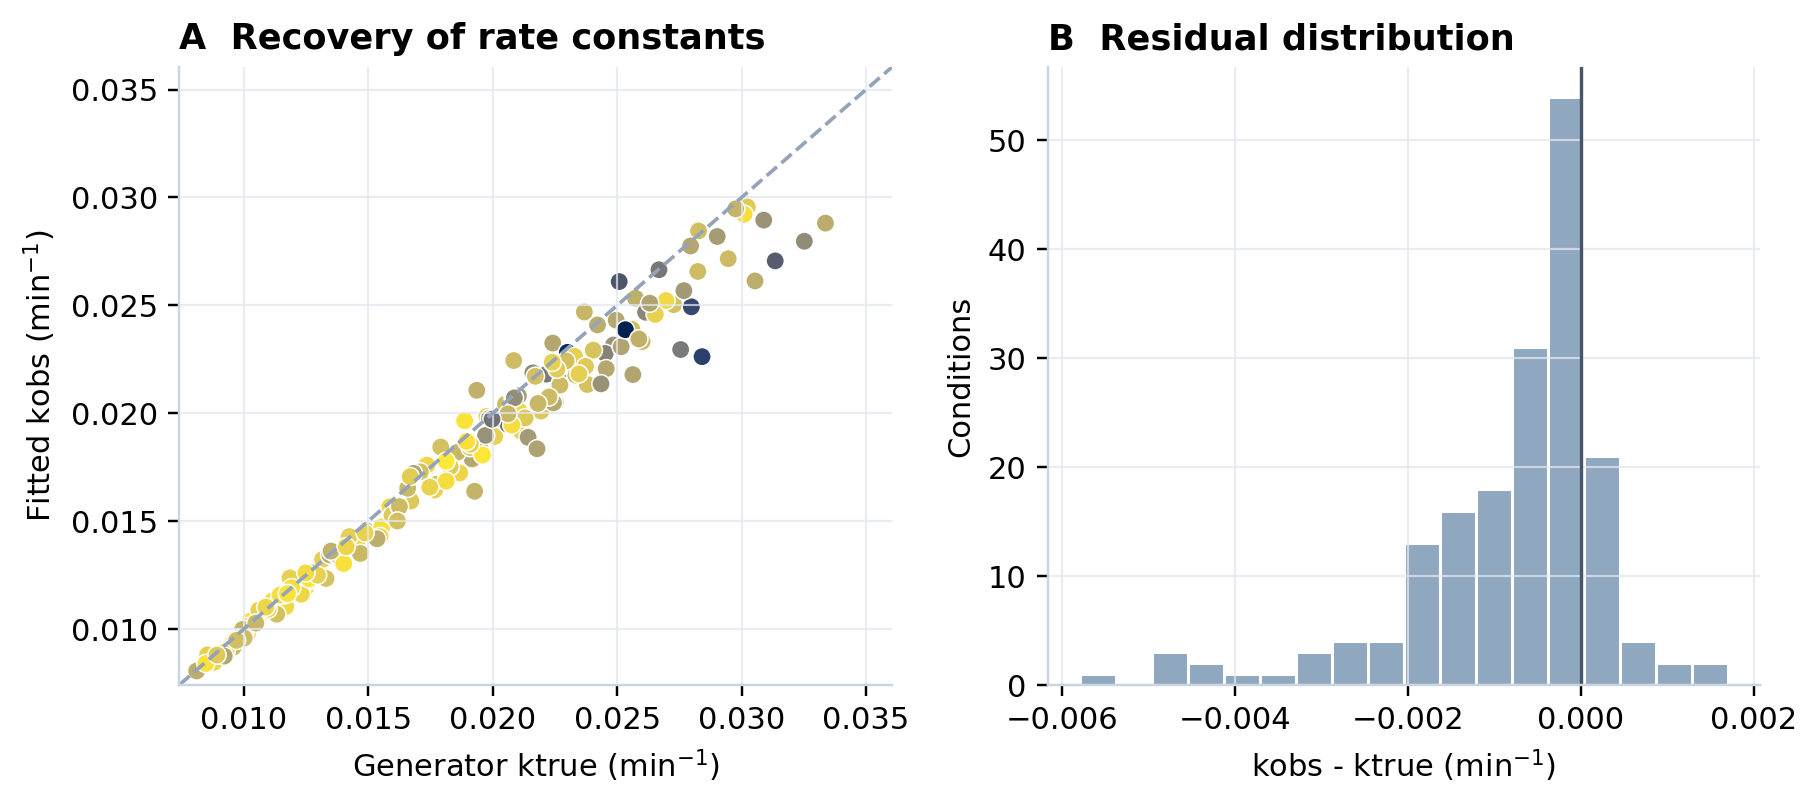
\includegraphics[width=0.95\linewidth]{../figures/figure3_diagnostics.png}
\caption{Kinetic fitting diagnostics. Left: fitted vs generator rate constants. Right: residual distribution.}
\label{fig:diagnostics}
\end{figure}

\section{Mechanistic Perturbation}
The radical-scavenger panel is included to mimic a common mechanistic check in photocatalysis papers. In the synthetic generator, IPA causes the strongest activity loss, followed by BQ and EDTA. This ordering is scripted and should not be read as real mechanistic evidence.

\begin{figure}[htbp]
\centering
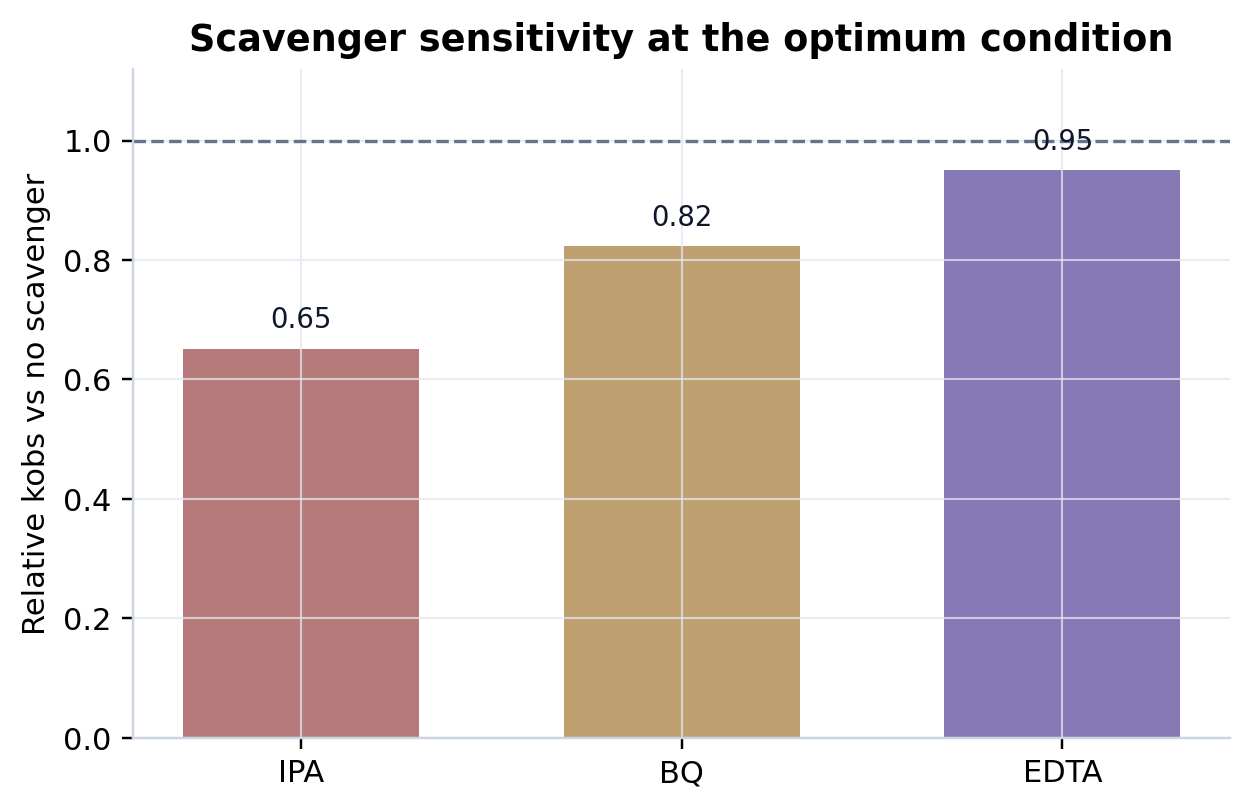
\includegraphics[width=0.74\linewidth]{../figures/figure4_scavenger_effects.png}
\caption{Synthetic scavenger sensitivity under the selected condition. Activity is normalized to the no-scavenger control.}
\label{fig:scavenger}
\end{figure}

\section{Reproducibility and Limitations}
Run \texttt{python scripts/run\_all.py} to regenerate the full project. A real English-journal submission would require actual experiments, instrument calibration metadata, replicate planning, uncertainty analysis, raw spectra, material characterization, and independent domain review. This artifact is a showcase of workflow shape and publication packaging.

\begin{thebibliography}{9}
\bibitem{fujishima1972} A. Fujishima and K. Honda, ``Electrochemical photolysis of water at a semiconductor electrode,'' \emph{Nature}, vol. 238, pp. 37--38, 1972, doi:10.1038/238037a0.
\bibitem{hoffmann1995} M. R. Hoffmann, S. T. Martin, W. Choi, and D. W. Bahnemann, ``Environmental applications of semiconductor photocatalysis,'' \emph{Chemical Reviews}, vol. 95, no. 1, pp. 69--96, 1995, doi:10.1021/cr00033a004.
\bibitem{pelaez2012} M. Pelaez, N. T. Nolan, S. C. Pillai, \emph{et al.}, ``A review on the visible light active titanium dioxide photocatalysts for environmental applications,'' \emph{Applied Catalysis B: Environmental}, vol. 125, pp. 331--349, 2012, doi:10.1016/j.apcatb.2012.05.036.
\bibitem{harris2020} C. R. Harris, K. J. Millman, S. J. van der Walt, \emph{et al.}, ``Array programming with NumPy,'' \emph{Nature}, vol. 585, pp. 357--362, 2020, doi:10.1038/s41586-020-2649-2.
\bibitem{virtanen2020} P. Virtanen, R. Gommers, T. E. Oliphant, \emph{et al.}, ``SciPy 1.0: fundamental algorithms for scientific computing in Python,'' \emph{Nature Methods}, vol. 17, pp. 261--272, 2020, doi:10.1038/s41592-019-0686-2.
\bibitem{hunter2007} J. D. Hunter, ``Matplotlib: A 2D graphics environment,'' \emph{Computing in Science \& Engineering}, vol. 9, no. 3, pp. 90--95, 2007, doi:10.1109/MCSE.2007.55.
\end{thebibliography}

\end{document}
